%% LyX 2.2.3 created this file.  For more info, see http://www.lyx.org/.
%% Do not edit unless you really know what you are doing.
\documentclass[english]{article}
\usepackage[T1]{fontenc}
\usepackage[latin9]{inputenc}
\usepackage{geometry}
\geometry{verbose,tmargin=0.05\paperheight,bmargin=0.05\paperheight,lmargin=0.1\paperwidth,rmargin=0.1\paperwidth}
\usepackage{amsmath}
\usepackage{graphicx}
\usepackage{setspace}
\usepackage{babel}
\usepackage{listings}
\renewcommand{\lstlistingname}{Listing}

\begin{document}

\title{Report - Assignment 2}

\author{- Akshay Anand (EE16B046)}
\maketitle
\begin{abstract}
\begin{singlespace}
In this week's assignment, $\int_0^x \frac{1}{1+t^2} dt$ was calculated
at different step-size $h$ for the variable $t$ using trapezoidal
integration method and the result was compared with the actual value
of the integral ($\tan^{-1}$x) and the result obtained using the
quad function in scipy.integrate module. The actual value of integral
($\tan^{-1}$x) was plotted for $0\leq x\leq5$ and compared with
the value obtained by the other 2 methods. Then, the maximum actual
and estimated error of values obtained using trapezoidal integration
method was plotted against decreasing $h$ value (step-size). The
error at different values of $x$ when using the quad function was
also plotted against $x$.
\end{singlespace}
\end{abstract}

\section{Function Definition}

The function to integrate ($\frac{1}{1+t^2}$) is initially defined.
\begin{lstlisting}
def function(t):     
	return 1/(1+t*t)
\end{lstlisting}

\section{Vector Initialisation}

A vector that covers the region: $0\leq x\leq5$ in steps of $h$
= 0.1 is initialised.

\begin{lstlisting}
h = 0.1 
x = np.linspace(0.0, 5.0, num=(5.0/h) + 1)
\end{lstlisting}

\section{Plot of $1/(1+t^{2})$ vs $t$}

The function $1/(1+t^{2})$  is now plotted against $t$.

\begin{lstlisting}
plt.plot(x, function(x)) 
plt.title('Plot of $1/(1+t^{2})$') 
plt.xlabel('t') 
plt.ylabel('$1/(1+t^{2})$') 
plt.show()
\end{lstlisting}

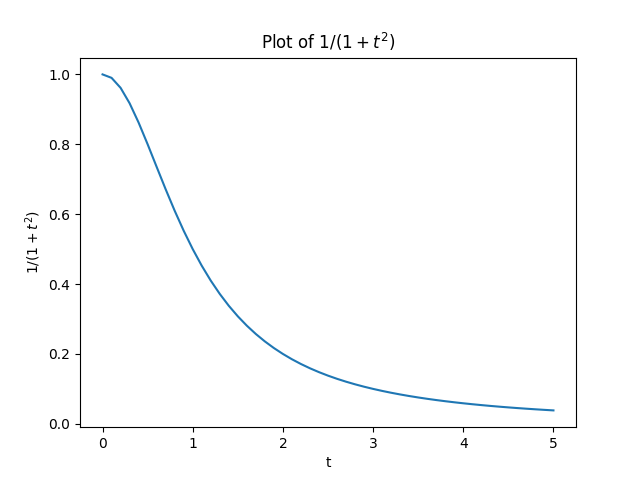
\includegraphics[scale=0.55]{initialPlot}

\section{Finding integral using scipy.integrate.quad}

The integral of the function $1/(1+t^{2})$ is now calculated from
0 to all values in the vector $x$ using scipy.integrate.quad and
its value is compared to the actual value of the integral i.e $tan^{-1} x$
and plotted in the same graph. The error between the two values is
also plotted against x.

\begin{lstlisting}
y = [] 
for i in x:     
	y.append(quad(function, 0, i)[0]) 
	df = pd.DataFrame() 		#df is a pandas DataFrame to tabulate the values
	df['tan^(-1) x'] = np.arctan(x) 
	df['Integral with quad'] = y 
	df.to_csv('quad_vs_tan^(-1).csv')

plt.plot(x, y, 'ro') 			#Plot the result of the integral
plt.plot(x, np.arctan(x), '#000000') 	#Plot the actual value of tan^(-1) x
plt.legend(('quad function','$tan^{-1} x$'))
plt.title('Integral plot using scipy.integrate.quad and actual value') 
plt.xlabel('x') 
plt.ylabel('$\int_0^x 1/(1+t^2) dt$') 
plt.show()
\end{lstlisting}

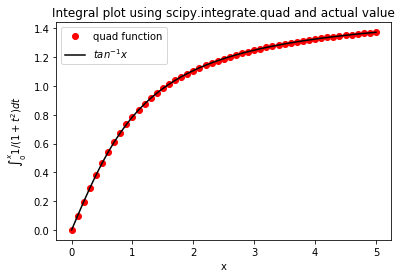
\includegraphics[scale=0.7]{quad}

The error is now plotted in a semi-log plot where error is in a logarithmic
scale and $x$, in linear scale.

\begin{lstlisting}

plt.semilogy(x, abs(y - np.arctan(x)), 'ro')
plt.title('Error plot between scipy.integrate.quad and actual value') 
plt.xlabel('x') 
plt.ylabel('Error') 
plt.show()
\end{lstlisting}

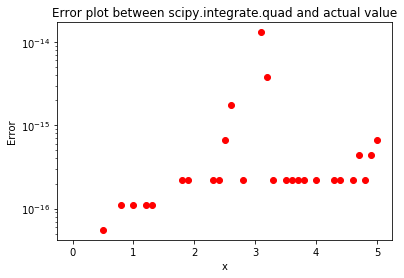
\includegraphics[scale=0.7]{errorQuad}

\section{Trapezoidal Integration}

Now, the value of the integral is found using the trapezoidal integration
method where the graph of the function is divided into thin trapezoids
of width $h$ (step-size) and the area of each is calculated and added
together to get the integral.

The formula used is: 
\[
I_{i}=h\left(\sum_{j=1}^{i}f\left(x_{j}\right)-\dfrac{1}{2}\left(f\left(x_{1}\right)+f\left(x_{i}\right)\right)\right)
\]

The value so obtained is now plotted in the same plot as the other
2 methods (actual value of $tan^{-1} x$ and quad method).

\begin{lstlisting}
def trapezoidalIntegral(h,a,b):     
	x = np.linspace(0.0, 5.0, num = (5.0/h + 1))     
	y = h*(np.cumsum(function(x)) - 0.5*(function(0) + function(x)))     
	return y

trapezoid = trapezoidalIntegral(0.1,0,5) 
plt.title('Integral plot using scipy.integrate.quad, actual value and trapezoidal integration') plt.xlabel('x') 
plt.ylabel('$\int_0^x 1/(1+t^2) dt$') 
plt.plot(x, np.arctan(x), 'g') 
plt.plot(x, y, 'ro') 
plt.plot(x, trapezoid, '+') 
plt.legend(('$tan^{-1} x$', 'quad function', 'Trapezoidal method'))  
plt.show()
\end{lstlisting}

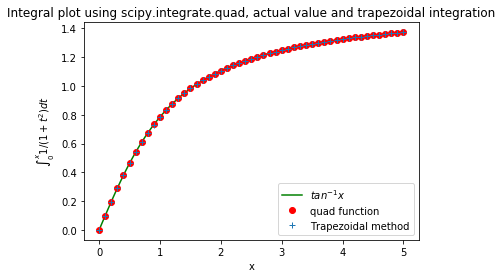
\includegraphics[scale=0.7]{triplePlot}

Now, the maximum actual and estimated error of the values obtained
using trapezoidal integration are plotted against step-size $h$.
The estimated error is calculated by subtracting the values obtained
by trapezoidal method at the same point at current step-size and half
its step-size while actual error is calculated as difference with
$tan^{-1} x$ at each point.

\begin{lstlisting}
estError = [] 
actError = [] 
h = 0.1 
hList = [] 
maxError = 1 
while maxError > 10**-8:       
	trapezoid = trapezoidalIntegral(h,0,5)     
	actError.append(max(abs(trapezoid - np.arctan(np.linspace(0, 5, num = (int)(5/h + 1))))))        
	hList.append(h)    
	h = h/2
	nextTrapezoid = trapezoidalIntegral(h,0,5)     
	maxError = max(abs(trapezoid - nextTrapezoid[::2]))     
	estError.append(maxError)

plt.loglog(hList, actError, 'ro') 
plt.loglog(hList, estError, '+') 
plt.title('Error plot') 
plt.xlabel('Step-size') 
plt.ylabel('Error magnitude') 
plt.legend(('Exact Error','Estimated Error')) 
plt.show()
\end{lstlisting}

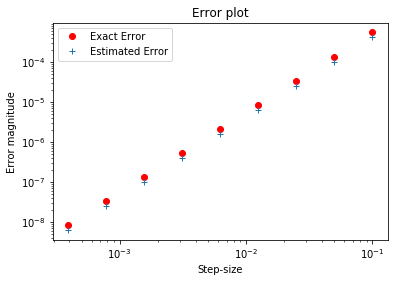
\includegraphics[scale=0.7]{errorFinal}
\end{document}
